\documentclass[sigconf]{acmart}

\usepackage{graphicx}
\usepackage{hyperref}
\usepackage{todonotes}

\usepackage{endfloat}
\renewcommand{\efloatseparator}{\mbox{}} % no new page between figures

\usepackage{booktabs} % For formal tables

\settopmatter{printacmref=false} % Removes citation information below abstract
\renewcommand\footnotetextcopyrightpermission[1]{} % removes footnote with conference information in first column
\pagestyle{plain} % removes running headers

\newcommand{\TODO}[1]{\todo[inline]{#1}}
\usepackage{endfloat}
\renewcommand{\efloatseparator}{\mbox{}}

\begin{document}
\title{Big Data Analytics in Monitoring  Outdoor Air Quality}


\author{Janaki Mudvari Khatiwada}

\affiliation{%
  \institution{Indiana University, Bloomington}
  \streetaddress{P.O. Box 1212}
  \city{Bloomington} 
  \state{Indiana} 
 \postcode{43017-6221}
}
\email{jmudvari@iu.edu}





\begin{abstract}
   Outdoor air pollution is one of the risk factors of public health. Air pollution adds burden to public health. Both developing and developed world use new technology and expertise to monitor outdoor air quality. 
   United States Environmental Protection Agency (USEPA) collects outdoor air quality data from state, local and tribal agencies through outdoor air quality monitors across the country. The data get collected into the Air Quality System (AQS) database. This data can be used for variety of purposes such as education, research and regulatory. Data from this data--mart is available for different time--series like hourly, daily, weekly, monthly and yearly. It gives us a real picture of outdoor air quality and measurements of pollutants present in the air in a particular time period. The data can be used for comparing air quality among different regions, raise awareness to general public so that they can play a role in reducing household air pollutants, to see the trend of air pollutants at different time periods in a day or a season, it can also be combined with emissions data for comparative study. Data analysis of pollutants help identify pollution hot spots. Since air quality is vital for public health and environmental health, air quality monitoring possesses great significance from public health perspective. It is worth looking at simple statistical values and level of air quality index value for the pollutants described as criteria pollutants as described by World Health Organizations. Simple statistical calculations in bigger datasets help understand the extent and source of problem. It helps in comparing past statistics with the present so helps in evaluations of action being taken during past periods. Looking at the overall mean value of criteria pollutants of 2016 and 2006 reveals improved air quality level to some extent for all core-based statistical areas. But the mean value of carbon monoxide has significantly increased over the ten years period.


\end{abstract}

\keywords{i523, hid330, Outdoor Air Quality, Big Data, Air Quality Index}


\maketitle



\section{Introduction}
   Outdoor air is a valuable natural resource that is vital to the health and existence of human beings and other forms of life. The outdoor air not only has clean air but has presence of various pollutants. Several health research have revealed that air pollutants are contributing factors for lung cancer, cardiovascular disease, acute and chronic respiratory conditions. World Health Organization (WHO) in 2013 has assessed that air pollution is carcinogenic to humans \cite{www-who}. ``In 2012 WHO estimated that 72 percent of outdoor air pollution-related premature deaths were due to ischaemic heart disease and strokes'' \cite{www-who}.
   Being aware of this fact, governments along with the scientists and the environmentalists help make policies to combat air pollution. Each country has set their own standards for outdoor air quality to protect their citizen's health. Every nation's standards depend upon their economic, cultural, social and political needs. ``The United States enacted its Clean Air Act (CAA) in 1970 and was amended in 1990 as a way to set stage for combating air pollution challenges'' \cite{epa-gov}. Since then, the country has made a lot of progress in improving air quality while sustaining a constant economic growth. After the enactment of CAA significant progress has been made in improving the outdoor air quality, reducing emissions levels from vehicles and power-plants. Over the period of 1990 and 2015, ``national concentrations of air pollutants improved 85 percent for lead, 84 percent for carbon monoxide, 67 percent for sulfur dioxide (1--hour), 60 percent for nitrogen dioxide (annual), and 3 percent for ozone'' \cite{epa-gov}. Particulate matters ``concentrations (24--hour) improved 37 percent and coarse particle concentrations (24--hour) improved 69 percent'' between 2000 and 2015 \cite{epa-gov}.
   Today, United States, European nations, India, China and other developing countries monitor outdoor air quality and use the collected data for identifying the particles present in the air, their contribution to various health problems, their sources, health research and also to find out the solutions to minimize their production level.

   Thousands of air quality monitors are placed  across the united States including US Virgin Islands and Puerto Rico. They are stationed based upon the significance of air quality effects on health.  These monitors stream outdoor air quality data to a national air database system called Air Quality System (AQS). As a result big outdoor air data is generated constantly everyday. Air Quality System database is a national database where state, local and tribal agencies submit all of the
   data collected from thousands of air quality monitors across the United States. These huge databases are easily accessible in EPAs air data website via AQS. Besides air data, AQS database system has
   weather and emissions data. Emissions data provides data from vehicular, industrial and powerplants emissions records. Weather plays an important role in the quality of outdoor air. For example, high wind may disperse concentration of chemical particles. AQS database also called AQS Data Mart, has summary of yearly air quality data since the year of 1957. These data give an understanding of outdoor air quality and different particles present in the air and their sources. Source of air particles can be natural or human generated. Pollen, smoke from wildfires, mold, dust are some of the natural air pollutants. Similarly, emissions from
   power--plants, industries and vehicles, different substances and solutions that human have generated for various purpose are human generated air pollutants. 

   To set standard for air quality, Air Quality Guidelines was published by WHO in 1987 and have been revised in 1997 \cite{who-health-topics}. WHO guidelines set an international standard for air quality based on which countries around the world set their own standards to achieve the goal set by WHO. 
   Nitrous Oxide (NO2), Sulphur dioxide (SO2), Carbon Monoxide (CO), ground level Ozone, Particulate Matter (PM) among others, are some of the common hazardous air pollutants. Particulate matters are categorized into two categories, PM2.5 and PM10, based on the size of fine particle. Based on the value of Air Quality Index (AQI), USEPA has classified Outdoor air quality, AQI level as `Good', `Moderate', `Unhealthy for sensitive Groups', `Unhealthy',
   `Very Unhealthy' and `Hazardous' \cite{airnow-gov}. The AQI value range from 0 to 500. The agency has assigned colors (`Green', `Yellow', `Orange', `Red', `Purple' and `Maroon' respectively) to each of the air quality categories \cite{airnow-gov}. It is shown in figure \ref{AQI}.

\section{Big Data and Outdoor Air Quality}
In US there are about 4,000 outdoor air quality monitors operated by state environmental agencies \cite{outdoor-air}. They constantly collect air data on harmful suspended particles present in the air and send them to a national database center which is
   AQS database. EPA has air quality database from last 27 years from around the states \cite{googlecloud}. The size of EPA's database is 25 GB. The data contains valuable information about the concentrations of different air pollutants in different time series; hourly, daily, weekly and yearly. Besides air quality data, AQS database also contains emissions data and weather data which are vital to the outdoor air air quality. Emissions data is basically data from vehicular and industrial emissions. They help to  understand the source of different air pollutants and their role in air quality as well as they can be used for furthering research in limiting their emissions. Yearly summary data of AQS Data Mart can also be used to see the progress made in reducing harmful air pollutants over the years. For example, EPA reported that emission of SO2 has reduced by 73 percent from 1990 to 2011 which is resulted primarily from electric utilities. Study of Emissions and air quality data gives an insight into the source of air pollutants and scientists can use these data to build a better industrial and vehicular models that reduces the emissions of pollutants. Similarly policy makers set vehicle emissions standards and industrial waste management. 

India and China, two bigger economies in the world are battling worst air pollution. In recent years IBM is doing collaborative work with local authorities to combat air pollution in cities like Delhi, Beijing and Johannesburg by providing its data analysis platform called `Green Horizons' \cite{www-huffingtonpost-com}. The platform uses machine learning tools to analyze past weather forecasts data along with near real time data from optical sensors, air quality monitors and satellites to understand past forecasting models and build a better prediction models for future forecasts \cite{www-huffingtonpost-com}. This prediction model helped Beijing enforce air quality control measures on traffic, construction and industry. 

Weather directly affects outdoor air quality. For example in a windy day PMs can easily be spread in a neighboring regions and high temperatures increases ground level ozone \cite{www-huffingtonpost-com}. Similarly, another example of relationship between big data analysis and air pollution is use of Microsoft's tools in incorporating Beijing's outdoor air data collected from conventional monitors along with data from ``environmental monitoring stations, traffic systems, weather satellites, topographic maps, economic data, and even social media '' \cite{spectrum-ieee}. 

Furthermore, OpenAQ is another platform besides EPA--AQS repository, which holds and hourly updates near--live air quality data from around the world. It claims to have ``collected 133,494,377 air quality measurements from 8,054 locations from 47 countries. Data are aggregated from 98 government level and research-grade sources'' \cite{googlecloud}. The platform helps general public identify global hotspots for poor air quality and allow to have a look at the outdoor air quality where they live \cite{googlecloud}. There is another open forum site called `Air--Now International' where users from around the world can participate in sharing and information about air quality data. ``It is an international version of USEPA's air now system''\cite{air-quality}. 
 Big volume of EPA's data can be combined with another big data, census data to find out the portion of population breathing polluted air. This gives an understanding of health effects among general public. Since, monitoring stations generate big volume of air pollution data and regularly stream into, EPA's open source, air database, any concerned individual can access live raw data from the website to find out about the quality of air they are breathing.  


\section{Air Pollutants}
EPA has prioritized six major air pollutants that are commonly found all over the US. They pose significant threat to public health and environment.  They are called `Criteria Pollutants' and they are ground level ozone, fine particles or particulate matter (PM2.5 and PM10), nitrogen dioxide, sulphur dioxide, lead and carbon monoxide \cite{epa-gov}. WHO has set the guidelines for each of these pollutants as shown in figure\ref{WHOGuidelines}.

PM2.5 are particles less than or equal to 2.5 micrometers in diameter while PM 10 are particles less than or equal to 10 micrometers. ``Sulfate, nitrates, ammonia, sodium chloride, black carbon, mineral dust and water are the main components of PM '' \cite{www-who}. These components combine with each other to form variety of mixtures in the air and can easily enter our lungs. Longer exposure to these substances increases the risk of lung cancer and cardiovascular disease \cite{www-who}. 

Data on emissions from powerplants, industries and motor vehicles shows that emitted pollutants like various volatile substances and various forms of nitrogen oxides (NO2) are responsible for the formation of ground level ozone. Chemical reactions between these substances create ground level ozone directly in the air \cite{epa-gov}. Chest pain, coughing, throat irritation and inflammation are common problems caused by ozone air pollution. The main source of NO2 is emissions from heating, power generation and engines in vehicles and ships. SO2 is another air pollutant produced mainly from burning of fossil fuels. Volcano is a natural resource so2 release  in the outdoor air. Longer exposure to this pollutant causes inflammation of respiratory tract \cite{www-who}. The data on these pollutants have been regularly analyzed to see their trend. They have also been used in health research to have an understanding of their impact on people's health. Keeping track of problems and source of problems help us in keeping problem at check. Some air pollutants are characterized as hazardous or toxic air pollutants. Some of the examples include benzene, cadmium, mercury, lead and asbestos. 

\section{Health Hazards}
Air pollutants, such as  hazardous air particles can easily reach our lungs when we breathe. The effects are itchy, irritated throat, nose and inflammation of respiratory tract. Pollutants such as PM 20 block our airtubes. These pollutants badly affects people with asthma and bronchitis. WHO had estimated that in 2012, 3 million premature deaths worldwide due to outdoor air pollution, particularly due to exposure to particulate matter of 10 microns or less \cite{www-who}. And in 2014 WHO has reported 7 million premature deaths worldwide \cite{www-who}. Other pollutants such as lead, pesticides, arsenic also called as toxic pollutants are carcinogenic hence are responsible for lung cancer which is one of premature deaths. Carbon monoxide a very common air pollutant generated by combustion has been called a silent killer. Its health effects include nausea, vomiting and reduced neuro and cardiovascular behavior as it blocks oxygen transfer inside the body thereby might lead to death without knowing the real cause of death. Exposure to higher level of ground level ozone have serious health issues, while it affects people with asthma and bronchitis, other groups of people also experience coughing, shortness of breath, eventually inflammation of airways and development of chronic obstructtive pulmonary disease \cite{ozone}.

Sulphur dioxide (so2) is a highly poisonous gas present in ambient air. It is a byproduct of burning of sulphur or product containing sulphur. Its main source is burning of fossil fuels especially in the powerplants and other industrial facilities. This pollutant can harm the environment by causing acid rain \cite{sulphur}. It harms human health by causing breathing difficulty and coughing. It combines with other particle pollutants present in the air causing haze. 

\section{Air Quality Index}
   AQI is the index, for five major air pollutants discussed above, calculated by special formula developed by EPA. EPA uses its own formula to convert daily concentrations of measurement of each pollutant into AQI value of each pollutant \cite{airnow-gov}. Among all the highest AQI value is reported as the daily AQI value for that day \cite{airnow-gov}.  Generally AQI 100 is the acceptable index set by EPA to protect public's health and it ranges from 0 to 500 \cite{airnow-gov}. The higher the value of AQI, greater is the pollution level and greater is the health risk. Based on hourly data collection from air quality monitors, stakeholders can constantly monitor AQI value in their cities or respective location. So weather channels in different media outlets such as local radio, television stations and newspapers also report about AQI index in order to inform general public about air quality in their area. Figure \ref{AQI} shows the AQI classification for each pollutant as recommended by WHO and implemented by U. S. EPA. EPA is requires to report any AQI value greater than 100 specifically in larger cities with population more than 350,000 \cite{airnow-gov}.


\section{Outdoor Air Quality Monitoring Stations}
   Outdoor(Ambient) air quality monitors are specified based on the significance of monitoring a particular pollutant \cite{air-quality}. The purpose might be to protect public health or environment in a densely populated areas. They might be stationed nearby, schools, hospitals, parks and recreational areas. While they are operated by several different agencies they are regulated by U. S. EPA. According to EPA these stations should meet all the requirements for designs and operations as regulated by EPA themselves. These stations not only provide data on air quality they help in evaluating the effectiveness of programs and policies on emissions control.


\section{WHO Guidelines and Clean Air Act}
   WHO guidelines for air quality is applied worldwide. This guidelines was revised in 2005 \cite{www-who}. The guidelines set standards for different air pollutants. According to the guidelines which is based on scientific evidence WHO has set standards for Ozone (o3), SO2, NO2 and PM. WHO guidelines try to limit the lowest possible values for these pollutants. For example WHO limit values for PM2.5 is 10 micrograms per cubic meter is annual mean and 25 micrograms per cubic meter is 24-hour mean and limit value for PM10 is 20 micrograms/m3 annual mean and 50 micrograms/m3 24-hour mean \cite{www-who} \ref{WHOGuidelines}. ``The 2005 WHO Air quality guidelines'' offer global guidance on thresholds and limits for key air pollutants that pose health risks. The Guidelines indicate that by reducing particulate matter (PM10) pollution from 70 to 20 micrograms per cubic metre, we can cut air pollution-related deaths by around 15 percent \cite{www-who}.

   United States' Clean Air Act (CAA), first enacted in 1970 and with major revisions in 1990, is a federal law which is defined as ``The Act that regulates air emissions from area, stationary, and mobile sources'' \cite{epa-gov}. CAA  . EPA is the administrator of CAA \cite{wikipedia-org}. As required by law, EPA regulates emissions standards for vehicles, industries, aircrafts and powerplants among others in order to protect environment and public health. Today, with the availability of new technology and analytical tools air quality data from the monitors across the regions can be accessed in an instant and can be analyzed for daily reporting.
   Based on daily AQI value, respective authorities can take appropriate actions to save outdoor air quality in areas where pollution level is insignificant and to identify measures to be taken in areas where air quality is poor.

\section{Methods}
\subsection{Air Quality Dataset}
   Outdoor air quality data sets are available in the USEPA.gov website called 'Air Data'. The data on 'Air Data website comes from AQS database where outdoor air data generated from thousands of air quality monitors from all over the country is collected. As mentioned, all states, local and private monitoring agencies send outdoor pollutants concentrations measurement data to the AQS database \cite{epa-gov}. Besides, Air Data there are other sources of data as well, they are briefly discussed below; 
\begin{itemize}
   \item 'Air Now' which
          has air quality forecasts and real--time data in visual form.

   \item `AirCompare' that has data about Counties' AQI summaries.
   \item `AirTrends' data is about trends of air quality and emissions.
   \item `Air Emissions Sources' has emissions data with national, state and county--level  summaries for criteria pollutant emissions.
   \item `Remote Sensing Information Gateway (RSIG)' that has air quality monitoring, monitoring and satellite data.
  \item `Air Data' datasets  have raw dataset,  AQI summary datasets. Summary reports consists of        AQI report which displays a yearly summary of AQI values in a county or city or Core     Based Statistical Area (CBSA). The AQI values are summarized by maximum percentile and median and count of days in each AQI category and the count of days when AQI could be attributed to each criteria pollutant \cite{epa-gov}.

  \item `` Quality Statistics Report has yearly summaries of air pollution values for a city or county. It shows the maximum values reported during the year by all monitors in CBSA or county'' \cite{epa-gov}.

  \item Monitor Values Report that has yearly summary of the measurements at individual monitors and has descriptive information about the site \cite{epa-gov}.

  \item Monitor Values Report-Hazardous Air Pollutants that shows HAPs summary data for individual monitoring sites \cite{epa-gov}.

  \item Air Quality Index Daily Values Report that has information about AQi values for specified year and location \cite{epa-gov}.
\end{itemize}

   The dataset that are being used for analysis are ``Daily AQI by CBSA 2016'' and ``daily AQI by CBSA 2006'', from EPA's air data website. Air data has different categories of outdoor air quality data. There are datasets for hourly as well as monthly time period broken down by single criteria pollutant of `Hazardous Air Pollutants' (HAPs). There are county level monitors and stations and datasets grouped by ``Core Based Statistical Area (CBSA)''. Each datsets have more than 17,000 data points. 

   CBSA is designed by Office of Management (OMB) as a geographical area that consists of one or more than one counties and similar surroundings that are associated with at least one core urbanized area of at least 10,000 population plus adjacent counties which are associated with each other in terms or social, economic and daily commutes \cite{www-census-gov}. CBSA collectively refers to Metropolitan and Micropolitan statistical areas. ``OMB defined Metropolitan and Micropolitan statistical areas in 2003 based on application of the 2000 standards with Census 2000 data. It became effective in 2003'' \cite{www-census-gov}. There are 922 CBSAs in total \cite{www-census-gov}. Metropolitan statistical areas are urbanized areas with population of 50,000 and its adjacent areas  while Micropolitan statistical areas are areas with population of at least 10000 or less than 50,000 \cite{www-census-gov}. 

   CBSA AQI datasets fits the scenario for monitoring outdoor air quality. Because the designed statistical areas are significantly populated along with higher concentrations of motor vehicles running, higher number of day to day activities, less natural habitats or and most of the areas are within industrial areas and powerplant generators. Also, the first look at the dataset give a general information about AQI value of each 'Criteria Pollutant' for a day in a year of each monitoring stations in CBSAs. 

\subsection{Methods}
   The comma separated dataset ``daily aqi by cbsa 2016'' was downloaded from data source ``https://aqs.epa.gov/aqsweb/airdata''. The dataset shows AQI value of each ``criteria pollutants'' for each CBSA recorded per day per station for the year 2016. Criteria pollutants recorded in the dataset are, PM2.5, PM10, Ozone, SO2, NO2 and CO. It also has a column for number of stations for each CBSA and location of the monitoring stations per CBSA. 

   In order to have a comparative study of any changes in AQI value for each parameter for the listed CBSA, dataset for the year 2006 is also being analyzed. This gives us a picture of changes if any for the duration of 10 years. Since real world datasets may not be perfect, there are slight or negligible amount of discrepancies among the two datasets.
   Criteria pollutants recorded in the dataset varies within each CBSAs depending on their significance in the region or monitoring stations. Similarly, record date per station per CBSA is not continuous, there are certain interval for recording and reporting data. For example, data is recorded on January 1st 2016 and the next date is January 3rd and 6th and so on. This pattern is seen in the whole dataset. Also, number of monitoring stations varies per CBSAs.

   Using jupyter notebook with python2.7 as the interpreter, the dataset is fetched and converted into pandas dataframe for  and analysis. Next, only the columns needed for analysis are   selected and created a clean pandas dataframe ready for manipulation. Jupyter Notebook is an open source web application which is powerful in data cleaning, manipulation, data analysis and visualizations. The notebook is not sufficient in itself for a variety of data manipulations, it needs to have all sorts of python packages as per requirement of data analysis. Matplotlib, pandas, numpy and pandas datetime are the packages used for air quality data analysis.  


\section{Analysis}
   The requirements for the analysis are python's jupyter notebook and the packages pandas, matplotlib and numpy. Using the pandas dataframe, average AQI value is calculated for each `Defining Parameter' grouped by CBSA.  Since AQI value determines the level of risk factor as shown in figure \ref{AQI}, it is worth calculating the mean of that value which helps in determining which CBSA is affected by which `defining Parameter'. It also helps identify the source of the pollutant so that responsible stakeholders can take required actions to solve the problem. The purpose of using the data set is to find out level of AQI per CBSA  for the year 2016. The reason of using 2016 data set is it the most recent complete set of data for a year. While 2017 data set would have been the most recent look at AQI level in the United States but as of this analysis the 2017 data set contains air quality data until the month of May 2017. This data set wold be completed as a full years data only in the upcoming spring \cite{outdoor-air}. In order to do a general comparison of the changes, positive or negative, if any similar data set for the year 2006 is selected. This would allow us to look at differences in AQI values in a decade time frame. 
\subsection{CBSA Average AQI for 2016}
   Simple statistical measures such as mean, maximum, count and minimum value for any variable provides some insights into the degree of variation between each measure of the variable within a period of time. So, as a first test mean value of ``Criteria Pollutants'' for all the listed CBSAs have been calculated. Then the results have been plotted into a bar--chart as shown in figure \ref{Average CBSA AQI 2016}. It shows that among all, Ozone and PM 2.5 have highest average among CBSAs while CO, NO2, SO2 and PM10 have slightly lower average AQI for the year 2016.  

   Furthermore, figure \ref{Top Ten Mean AQI Value for the Year 2016} illustrates the average AQI value for overall CBSAs for the year 2016 by month. The table illustrates that AQI value, which is 53.56, for Ozone is the highest during the month of June of last year. This AQI value of ozone comes under the category of`unhealthy for sensitive groups'. This value is followed by CO which has the highest mean value for two consecutive months, May and June. From the table it can be said that during 2016 the most significant criteria pollutants were Ozone, CO, and PM2.5.

   In order to look at monthly average AQI per `Defining Parameter', first 'Date' series is converted into pandas datetime format and then the series is bucketed into month of the year column. Then mean is calculated by using `groupby' function, mean is calculated grouped by `Defining Parameter' and `month of year'. The result illustrated in figure \ref{Mean AQI per Month 2016} shows that there is no  significant change in mean AQI for SO2 and PM10 while significant change can be seen for CO and Ozone. AQI average for CO shows a sharp increase in May. 

   For the purpose of finding out CBSA with highest and lowest average  AQI value for the year 2016, for specified pollutant, aggregate function is used with groupby function with descending value of AQI. The result is shown in figure \ref{Lowest Mean AQI per CBSA 2016}. The table shows CBSA `Madison, WI' has lowest AQI value for SO2, followed by Fayetteville, NC for the same parameter.
   Similarly, as seen figure \ref{Highest Mean AQI per CBSA 2016} Hilo, Hawaii has the highest AQI value for parameter SO2 which is 151.79. This means AQI value is unhealthy and people may experience health effects with sensitive groups people with asthma, bronchitis and chronic obstructive pulmonary disease (COPD) might have very serious health effects as stated in figure \ref{AQI}. The reason for highest AQI value for SO2 might be the release of SO2 gas from active volcanoes around the CBSA region as SO2 is one of the gases released from volcanoes. Hilo, HI is followed by `Riverside-- San Bernardino--Ontario, CA with AQI value 126.53 for  \ref{AQI} with category `unhealthy'. Other CBSAs in the top ten list are Lansing--East Lansing, MI, San Juan--Carolina--Caguas, PR, Bishop, CA, Durango, CO, Riverside--San Bernardino--Ontario, CA, Philadelphia--Camden--Wilmongton, PA--NJ--DE--MD, Los Angeles--Long Beach--Anaheim, CA and Minneapolis--St.Paul--Bloomington, MN--WI. All of these CBSAs have at least one defining parameter with `Unhealthy' AQI value. It is also significant that Riverside--San Bernardino--Ontario, CA have two highest AQI value for two defining parameters that is ozone and PM 10.

   In order to have a visual picture of level of AQI value, count measure is used grouped by `CBSA', `Defining Parameter' and `Category' and visualized the result in a boxplot. This basically counted number of days in each category of AQI. The figure \ref{boxplot} shows, that there are significant number of `good days' during 2016 followed by `moderate', `unhealthy for sensitive groups' and rest of the three categories have less range of days. As seen in bar chart the mean value for Ozone is higher for the months May and August in comparison to other pollutants Columns for the months of June and July are missing at this point.


\subsection{Comparative AQI for 2006 and 2016}

   To compare AQI per CBSA for criteria pollutants, exactly similar data set for the year 2006 is used to calculate average AQI value and plotted into a bar chart which is shown in figure \ref{Average CBSA AQI 2006}. As the result can be compared with that of 2016.
   average AQI  value for ozone and SO2 is significantly higher compared to 2016 while that of carbon monoxide (CO) has increased significantly from 2006 to 2016. For other parameters there are not so significant changes. Similarly, average AQI for SO2 is also higher in 2006 compared to 2016. 
   There is also some changes in overall average AQI vlaue. This figure shown here \ref{Top Ten Mean AQI Value for Year 2006} illustrates the AQI average for the year 2006. As seen in barplot this figure shows the highest mean for Ozone at the top of the list when mean is grouped by month of the year and output is sorted in descending order by mean. Interestingly, most of the highest mean value are for the month of June, July and August. To be more specific AQI value for Ozone is mostly during above listed months. Similar result can also be seen in the  analysis of 2016 dataset.

   While comparing top ten CBSA with highest average AQI value for 2016 with that of 2006, top ten CBSAs with highest average AQI for 2006 is shown in figure \ref{Mean AQI per Month 2006}. Compared to 2016 there is no sharp increase in mean value for CO any of the month as has been in 2016. Its mean value remains comparatively in same range, in between 17 and 16. Whereas, the value for Ozone is significantly higher for teh months of March, April, May, August and September. For other months as well it has higher level o mean AQI compared to other pollutants except for SO2 which has the second highest AQI throughout the months. Average value for all of the pollutants throughout the months have higher values compared to that of year 2016 except for CO. Average CO AQI for 2016 is higher than that of the year 2006. 

   Another comparison can be done by looking at the list of top most CBSAs with higher mean AQI. We have already discussed about this for year of 2016.  Now we will look at similar output for 2006 which is shown in figure \ref{Highest Mean AQI per CBSA 2006}. The mean output is generated by grouping the CBSA and defining parameter. Here, Bishop, CA has highest yearly average for PM10 which is 435.21 followed by CBSA Phoenix-Mesa-Scottsdale, AZ, Carlsbad-Artesia, NM have yearly mean value of 127 for SO2. In comparision to the same statistics for year2016,  mean value is lower than that of 2006. This indicated that there is progress made in lowering the measurement in air pollutant.




\section{Further Studies}
   It would be effective to look at the factors that helped lower the mean AQI value within a decade. Are there any policy differences between now and then? Are there less economic activities compared to 2016 or did any of the technology have any role to play to make such change? It would be effective to look at the factors that helped lower the mean AQI value within a decade. As can be see from the analysis above average ozone has highest average value among all. Finding out or looking at the contributing factors can be another area of furthering this research. and it would be interesting to see any changes if any during the year of 2017. The analysis presented here showcases just the level of pollutants by AQI value. For furthering the studies different models for lowering AQI value for a single pollutant within certain periods of time can be developed. Since vehicular, industrial or air transportation emissions are some of the main sources of criteria pollutants, it would be very effective to analyze monthly emissions data with AQI data to have an understanding of level of pollutants generated from these sources. This analysis can be combined with weather data in order to find out the effects of weather or seasonal variations on increasing or lowering pollutants. There is an increased AQI value for CO from 2006 to 2016. Factors responsible for poor AQI value can be the next research topics. 
   
   Looking at difference in emissions policy during the past decade will also provide some insight into why certain parameters have lower AQI value. Looking at effects of AQI value in international boundaries that is effect evaluation of pollutants of country affecting the air quality of surrounding country could be a whole new topic of outdoor air quality study.



\section{Conclusion}
   
   Air quality monitors across the United States and its territories, Puerto Rico and Virgin Islands collects everyday air data in order to collect data on pollutants present in outdoor air. These generates a  huge volume of data. Air data contains measurements of concentrations of pollutants, commonly called as criteria pollutants, present in outdoor air. These monitors are under the management of state, local or private environmental agencies. They collectively send these data to a national database system called air quality system. For analytical purpose the air data from the AQS website which is an source of air data, is directly accessed through jupyter notebook. Simple statistical measures are calculated to have a look at the level of pollutants present in ambient year.
   
   The  air data by CBSA, for the year of 2016  have been analyzed to see the average value of AQI for each defining parameter or criteria pollutants. This analysis identifies that average AQI value for Ozone is significantly higher compared to other pollutants. The analysis also shows that AQI value varies by month of the year. The results shows that Ozone AQI is higher in the months of March to August. While calculating overall average AQI, among all of the criteria pollutants level of ground level ozone has the highest value during the year of 2016 as well as 2006. It can also be concluded that overall level of AQI value have been improved over the years period while comparing the value from 2006 with that of 2016. Interesting enough AQI value of CO have been significantly increased from 2006 to 2016.
   
   Air quality monitoring have become an important and effective policy for reducing the concentrations of different criteria pollutants. Since the adoption of clean air act 
   in United States significant progress has been made in improving outdoor air quality.
   Thereby reducing the development of health risk factors for general public. Air quality monitoring stations collect everyday measurement values of criteria pollutants which generates a big volume of air data. This gives us information on daily level of pollutants present in the air thereby letting us know the quality of air that we breathe everyday. This information is shared to the public through various media outlet. This raise awareness among general public about the importance of outdoor air and their health.
   
  
  
\begin{acks}

  The author would like to thank Dr. Gregor von Laszewski for his motivating words and attitude and support to achieve our best. Also I would like to express my gratitude to teaching assistants Juliette Zerick, Saber and Miao for their encouraging attitude and technical support and suggestions while writing this paper.
  

\end{acks}

\bibliographystyle{ACM-Reference-Format}
\bibliography{report} 

\begin{figure}[htb]
\includegraphics[width=1.0\columnwidth]{images/sourceandhealtheffects.png}
  \caption{WHO Guidelines Source And Health Effects \cite{guidelines}}
  \label{WHOGuidelines}
\end{figure}

\begin{figure}[htb]
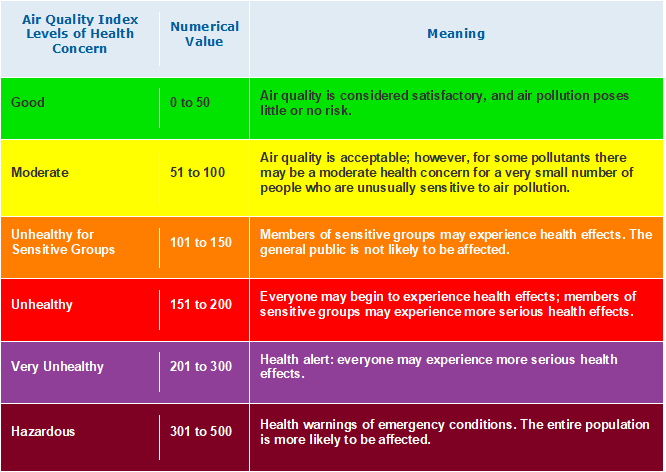
\includegraphics[width=1.0\columnwidth]{images/aqiclassification.png}
  \caption{Air Quality Index \cite{airnow-gov}}
  \label{AQI}
\end{figure}


\begin{figure}[htb]
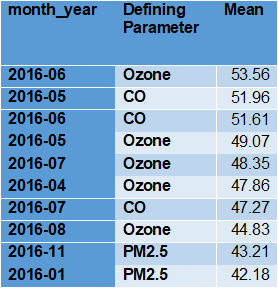
\includegraphics[width=1.0\columnwidth]{images/top10meanaqi2016.png}
  \caption{Top Ten Mean AQI Value for the Year 2016}
  \label{Top Ten Mean AQI Value for the Year 2016}
\end{figure}

\begin{figure}[htb]
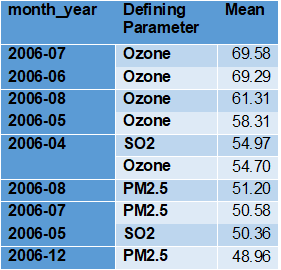
\includegraphics[width=1.0\columnwidth]{images/top10meanaqi2006.png}
  \caption{Top Ten Mean AQI Value for the Year 2006}
  \label{Top Ten Mean AQI Value for Year 2006}
\end{figure}


\begin{figure}[htb]
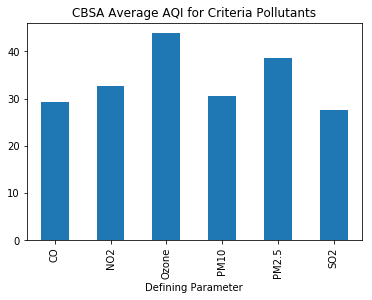
\includegraphics[width=1.0\columnwidth]{images/averageaqi2016.png}
  \caption{CBSA Average AQI for Criteria Pollutants}
  \label{Average CBSA AQI 2016}
\end{figure}

\begin{figure}[htb]
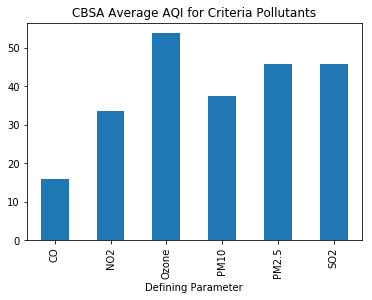
\includegraphics[width=1.0\columnwidth]{images/averageaqi2006.png}
  \caption{CBSA Average AQI for Criteria Pollutants 2006}
  \label{Average CBSA AQI 2006}
\end{figure}

\begin{figure}[htb]
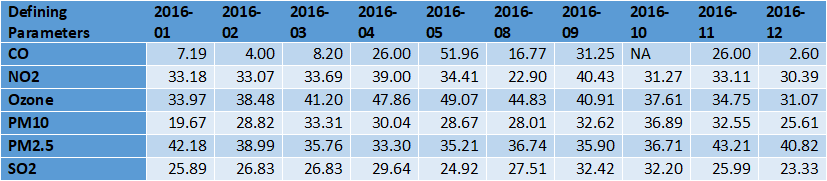
\includegraphics[width=1.0\columnwidth]{images/avaqibymonth2016.png}
  \caption{ Mean AQI per Month per Criteria Pollutant 2016}
  \label{Mean AQI per Month 2016}
\end{figure}


\begin{figure}[htb]
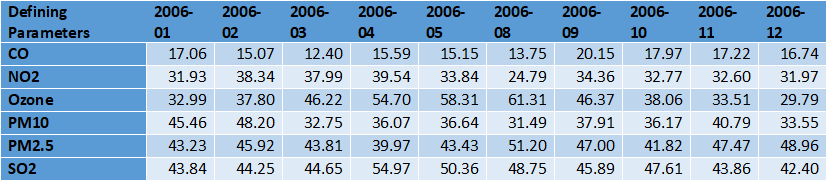
\includegraphics[width=1.0\columnwidth]{images/avaqibymonth2006.png}
  \caption{ Mean AQI per Month per Criteria Pollutant 2006}
  \label{Mean AQI per Month 2006}
\end{figure}


\begin{figure}[htb]
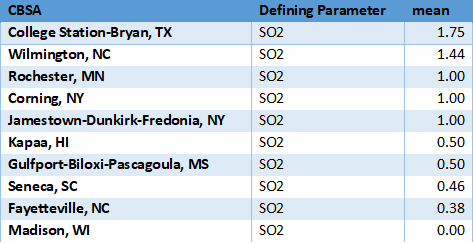
\includegraphics[width=1.0\columnwidth]{images/lowestmeanaqipercbsa.png}
  \caption{Lowest Mean AQI per CBSA 2016}
  \label{Lowest Mean AQI per CBSA 2016}
\end{figure}

\begin{figure}[htb]
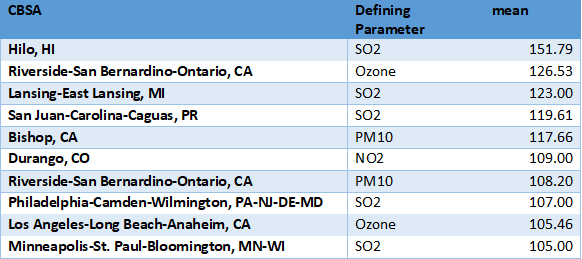
\includegraphics[width=1.0\columnwidth]{images/cbsahighestaqi.png}
  \caption{Highest Mean AQI per CBSA 2016}
  \label{Highest Mean AQI per CBSA 2016}
\end{figure}

\begin{figure}[htb]
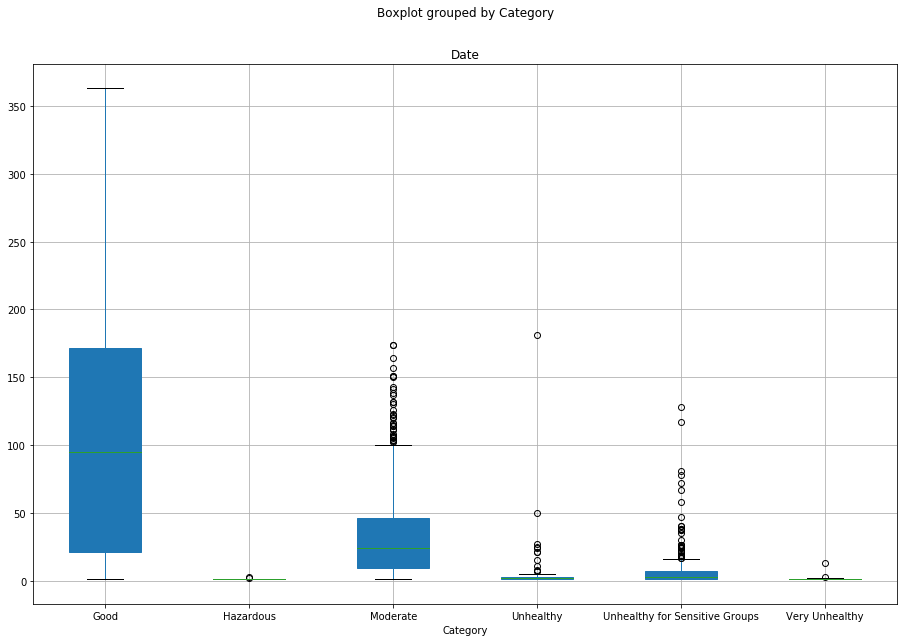
\includegraphics[width=1.0\columnwidth]{images/boxplotofcountofaqibycategory2016.png}
  \caption{Boxplot Grouped by Category, 2016}
  \label{boxplot}
\end{figure}

\begin{figure}[htb]
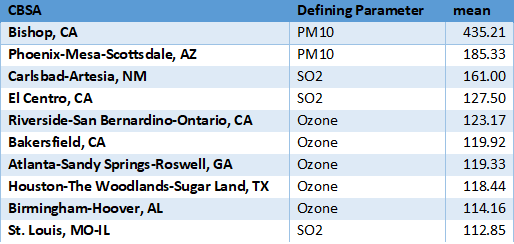
\includegraphics[width=1.0\columnwidth]{images/top10cbsamean2006.png}
  \caption{Highest Mean AQI per CBSA 2006}
  \label{Highest Mean AQI per CBSA 2006}
\end{figure}






\end{document}
